\documentclass[11pt]{article}
\usepackage{fullpage}
\usepackage{graphics}

\def\VERSION {0.8d}
\def\DEFAULTPORT {6665}
\def\HOMEPAGE {{\tt http://playerstage.sourceforge.net}}

\begin{document}
\setcounter{page}{0}
\pagenumbering{roman}

\titlepage

\begin{tabular}{lcr}
  \begin{tabular}{c}
	Player/Stage project\\
        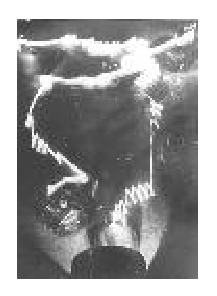
\includegraphics{notext_ps_logo}
   \end{tabular}
  &
  \hspace{5cm}
  &
  \begin{tabular}{r}
    {\bf USC Robotics Laboratory}\\
    University of Southern California\\
    Los Angeles, California, USA\\
  \end{tabular}
\end{tabular}

\vspace{5cm}
\centerline{\huge{{\em Old} C++ Client}}
\vspace{0.5cm}
\centerline{\large{Version \VERSION\ Reference Manual}}
\vspace{2cm}

\centerline{\large Brian P. Gerkey\\ Kasper St\o{}y}
\vspace{1cm}

\centerline{This document may not contain the most current documentation on} 
\centerline{the {\em Old} C++ client.  For the latest documentation, consult:}
\centerline{\HOMEPAGE}

\vspace{4cm}

\centerline{\today}

\newpage
\tableofcontents
\newpage

% reset page number to start with 1
\setcounter{page}{0}
\pagenumbering{arabic}
\section{The {\em Old} C++ Interface}
\label{app:oldc++}
{\Large \bf This manual describes the now obsolete (and largely non-functional)
C++ client library that was included with versions of Player prior to 0.9.
The documentation is provided here for convenience only; new control programs
should definitely use the new C++ client library; consult {\em Player C++
Client Library Reference Manual}}.

\subsection{Hello World}

This is a short tutorial that explains how to use the Player robot
 server using the provided interface written in C++. The source
 code is available in playerclient.h and playerclient.cc and is 
included in the Player distribution.

The source code shown in Figure~\ref{helloworld} is a complete
program that makes the robot move around doing very limited obstacle 
avoidance.
Let's go through the code step by step to get a feeling for what
it does. All the code needed to interact with the Player server is
wrapped into the C++ class CRobot. 

The method {\tt Connect(``tanis'')} sets up the connection to the server
running on the host ``tanis'' using TCP/IP. This method will
return non-zero if it fails to setup the connection; a meaningful
error statement will be printed to stderr.
After that we call {\tt Request( "srpw" )}.
This request tells Player what data we need access to. In this
case we want read ({\tt r}) access to the sonars ({\tt s}) and write ({\tt w})
access to the position device\footnote{This is the device used to 
control the robots wheels}. This tells the server to start sending
sonar data to the client continuously\footnote{The default rate is 
10Hz.} and accept position commands from the client. The program now
goes into a read-act-write loop for one thousand iterations. {\tt 
Read();} blocks and waits for the server to send
the sonar data.
The sonar data is then printed to the terminal using the {\tt Print()}
method. The client calculates and sets the variables {\tt newturnrate} and
{\tt newspeed} in the robot object based on the sonar data. Finally {\tt 
Write()} is called. This method writes the commands that the client has 
permissions to write to the server; in this case the newspeed and 
newturnrate. After the one thousand iterations has been reached another
request is send. This time the request is to close ('c') the access to
the position and sonar device. That's it.

\begin{figure}
\begin{verbatim}
#include <playerclient.h>

int main(int argc, char *argv[]) {
  CRobot robot;

  // where tanis is the hostname of the robot
  if(robot.Connect("tanis"))
    exit(1);

  if(robot.Request("srpw")) 
    exit(1); 

  for(int i=0;i<1000;i++) 
  {
    if(robot.Read())
      exit(1);

    robot.Print();

    if((robot.sonar[0] + robot.sonar[1]) < 
       (robot.sonar[6] + robot.sonar[7])) 
      robot.newturnrate = -20; // turn 20 degrees per second
    else
      robot.newturnrate = 20;
 
    if(robot.sonar[3] < 500) 
      robot.newspeed = 0;
    else 
      robot.newspeed = 100;
 
    robot.Write();
  }

  /* close everything */
  robot.Request("scpc");

  return(0);
}
\end{verbatim}

\caption{ ``Hello world'' code for the Player robot server.}
\label{helloworld}
\end{figure}

\subsection{Connecting}

The connection is created using
the {\tt Connect} method. There are actually three forms of this
method:

\begin{verbatim}
  int CRobot::Connect();
  int CRobot::Connect(char* host);
  int CRobot::Connect(char* host, int port);
\end{verbatim}

The first form, with no arguments, will connect to the Player server running
on the host and TCP port specified by the public (and thus user-modifiable) 
fields {\tt CRobot::host} and 
{\tt CRobot::port} (defaults are ``localhost'' and \DEFAULTPORT, respectively).  
The next two forms allow the caller to override the host and port.

If there is any error, {\tt Connect()} will return non-zero, and
the connection to the server has not been established.  Otherwise,
it returns zero.


\subsection{Request}

The request is made using the {\tt Request()}
method. 
for details on the format of the request string (which must be
NULL-terminated).
\begin{verbatim}
  int CRobot::Request(char* request_string)
\end{verbatim}

If there is any error, {\tt Request()} will return non-zero;
some parts of the request may have been accepted and processed
by the server, but certainly at
least one part was not.  Otherwise, it returns zero.


\subsection{Read}

After requesting access to some sensors, the user can call the following
method:

\begin{verbatim}
  int CRobot::Read()
\end{verbatim}

This method will block until it has received data from all the sensors
for which read access was requested and granted.  If there
is some error, it will return non-zero; otherwise it will
return zero and the received data is placed
into various data structures in the {\tt robot} object (see the source
code for more details):

\begin{verbatim}
  struct CGripper {
    /* gripper attributes */
    unsigned char paddlesOpen;
    unsigned char paddlesClose;
    unsigned char paddlesMoving;
    unsigned char paddlesError;
  
    unsigned char leftPaddleOpen;
    unsigned char rightPaddleOpen;
  
    unsigned char gripLimitReached;
   
    unsigned char liftUp;
    unsigned char liftDown;
    unsigned char liftMoving;
    unsigned char liftError;
  
    unsigned char liftLimitReached;
  
    unsigned char outerBeamObstructed;
    unsigned char innerBeamObstructed;
  };
  
  struct CMisc {
    /* misc attributes */
    unsigned char frontbumpers;
    unsigned char rearbumpers;
    unsigned char voltage;
  };

  struct CPtz {
    /* ptz attributes */
    short pan;
    short tilt;
    short zoom;
  };
  
  struct CPosition {
    /* Position information */
    unsigned int time;
    int xpos, ypos;
  
    unsigned short heading;
    short compass;
    short speed, turnrate;
    unsigned char stalls;
  };

  struct CBlob {
    /* data for a single color blob */
    unsigned int area;
    unsigned char x;
    unsigned char y;
    unsigned char left;
    unsigned char right;
    unsigned char top;
    unsigned char bottom;
  };
  
  struct CVision {
    /* this array, indexed by channel, tells the number of blobs detected
     * on that channel*/
    char NumBlobs[ACTS_NUM_CHANNELS];

    /* this array, indexed by channel, contains the blob data for each
     * blob detected on that channel */
    CBlob* Blobs[ACTS_NUM_CHANNELS];
  };

  class CRobot {
   /* (some parts left out here) */
   public:
    /* data from robot */

    /* sonar data is a 16-element array 
     * the sonars number from 0 at the front left of the robot clockwise
     * around to number 15 at the back left */
    unsigned short *sonar;

    /* laser data is a 361-element array 
     * the laser scans number from 0 at the right side of the laser
     * counterclockwise to 361 at the left side */
    unsigned short *laser;

    CPosition *position;
    CVision *vision;
    CGripper *gripper;
    CMisc *misc;
  }
\end{verbatim}
      
  
\subsection{Command}

The user is protected from all the byte manipulation needed to send commands.
The user sets variables in the class corresponding to the commands and
then when all command variables have been set the method {\tt Write()} is used. 
{\tt Write} checks what write permissions the client has and write the commands
the client is allowed to write to Player.

%\begin{figure}
\begin{verbatim}
  class CRobot {
    /* (some parts left out here) */
    public:
    /* commands to robot */

    /* new forward velocity, mm/sec, positive is forward */
    short newspeed;

    /* new turnrate, deg/sec, positive is counterclockwise */
    short newturnrate;

    /* new absolute camera positioning
     *   pan  : -100 to 100 degrees, positive is counterclockwise 
     *   tilt : -25 to 25 degrees, positive is up
     *   zoom : 0 to 1023, 0 is wide and 1023 it telefoto */
    short pan;
    short tilt;
    short zoom;

    /* new gripper command (see below) */
    short newgrip;
  }
\end{verbatim}

To aid the user in controlling the gripper, the following method is 
provided:

\begin{verbatim}
  void CRobot::GripperCommand( unsigned char command )
  void CRobot::GripperCommand( unsigned char command, unsigned char value )
\end{verbatim}

This method is used to set the command field {\tt newgrip} 
properly\footnote{Note that {\tt GripperCommand()} does not send
any commands to the robot; the user must still call {\tt Write().}}.  
The first form is used when the desired command requires no argument; 
the second form is used for gripper commands that 
do require an argument.  Examples (see the Gripper manual and read
the source for more details):

\begin{verbatim}
  robot.GripperCommand( GRIPPress, 20 );
  robot.GripperCommand( GRIPclose );
\end{verbatim}

\subsection{Configuration}
The CRobot class supports the following methods for configuring the 
server:

\begin{verbatim}
  int CRobot::SetDataMode(data_mode_t mode);
  int CRobot::SetFrequency(unsigned short freq);
  int CRobot::RequestData();
  int CRobot::ChangeMotorState(unsigned char state);
  int CRobot::ResetPosition();
  int CRobot::ChangeVelocityControl(velocity_mode_t mode);
\end{verbatim}

These methods should only be called after a successful call to
{\tt Connect()}.  In all cases, they return non-zero on error
(the configuration change was not made) and zero otherwise.

The argument to {\tt SetDataMode()} should be either {\tt REQUESTREPLY}
to put the server into request/reply mode or {\tt CONTINUOUS} to 
put it into continuous mode. When in request/reply mode,
{\tt RequestData()} requests one round of sensor data from the server.
When in continuous mode, {\tt SetFrequency()} allows
the user to set the continuous data rate to any frequency (in Hz). 
The default behavior of the server is to operate in continuous mode
at a frequency of 10Hz. 

Whereas the three previous methods will have their expected effect
if they are called any time after a call to {\tt Connect()}, the
following three methods will only make a change if one of the
microcontroller-mediated devices (currently position, sonar, miscellaneous,
and gripper) has already been successfully requested.
If the argument to {\tt ChangeMotorState()} is zero, the motors
are disabled (powered off); otherwise they are enabled (be VERY careful
when turning the motors on from software!).  The {\tt ResetPosition()}
method takes no arguments, and simply resets the robot's 
odometry to $(x,y,heading) = (0,0,0)$.
 The argument to {\tt ChangeVelocityControl()}
method should be either {\tt DIRECTWHEELVELOCITY} to use direct-wheel
velocity control or {\tt SEPARATETRANSROT} to use separate
translational and rotational velocity control; the default is to
use direct-wheel velocity control.

\end{document}
